\chapter{Collaborating on a Drupal site}

Throwing your codebase into Git or an other versioning system will not be enough to enable you to collaborate on your Drupal site. Since Drupal uses a database to store its contents this database should be shared as well. In this course we recommend using the OpenShift cloud for hosting your site.
OpenShift is a platform as a service product from Red Hat. The software that runs the service is open-sourced under the name OpenShift Origin, and is available on GitHub. Developers can use Git to deploy web applications in different languages on the platform. A version for cloud computing is named OpenShift Enterprise. OpenShift also supports binary programs that are web applications, as long as they can run on Red Hat Enterprise Linux. This allows the use of arbitrary languages and frameworks. OpenShift takes care of maintaining the services underlying the application and scaling the application as needed.

\section{Creating an openshift account}

\begin{itemize}
	\item First go to \url{https://www.openshift.com/}
	\item Click on \textbf{Sign Up}
	\item Fill out your information
	\item Click \textbf{Sign Up}
	\item Verify your account
	\item Accept the terms of service
	\item Click \textbf{Create your fist application now}
\end{itemize}

OpenShift gives you the option to create an instant Drupal 7 app. Since we are using Drupal 8 we will not use this option. We are going to create a PHP 5.4 application. This is a Linux server running a PHP web hosting environment. Click the PHP 5.4 application link and enter the following information:

\begin{description}
	\item[Public url] drupalsite-[firstname][lastname].rhcloud.com
	\item[Source code] leave empty
	\item[Scaling] No scaling
	\item[Region] aws-us-east-1
\end{description}

Click the \textbf{Create application} button.

When OpenShift asks if you will be changing the code for the application, click \textbf{Not now, continue}. You will see a page like figure \ref{fig:openshift_applications_overview}.

\begin{figure}[H]
	\centering
	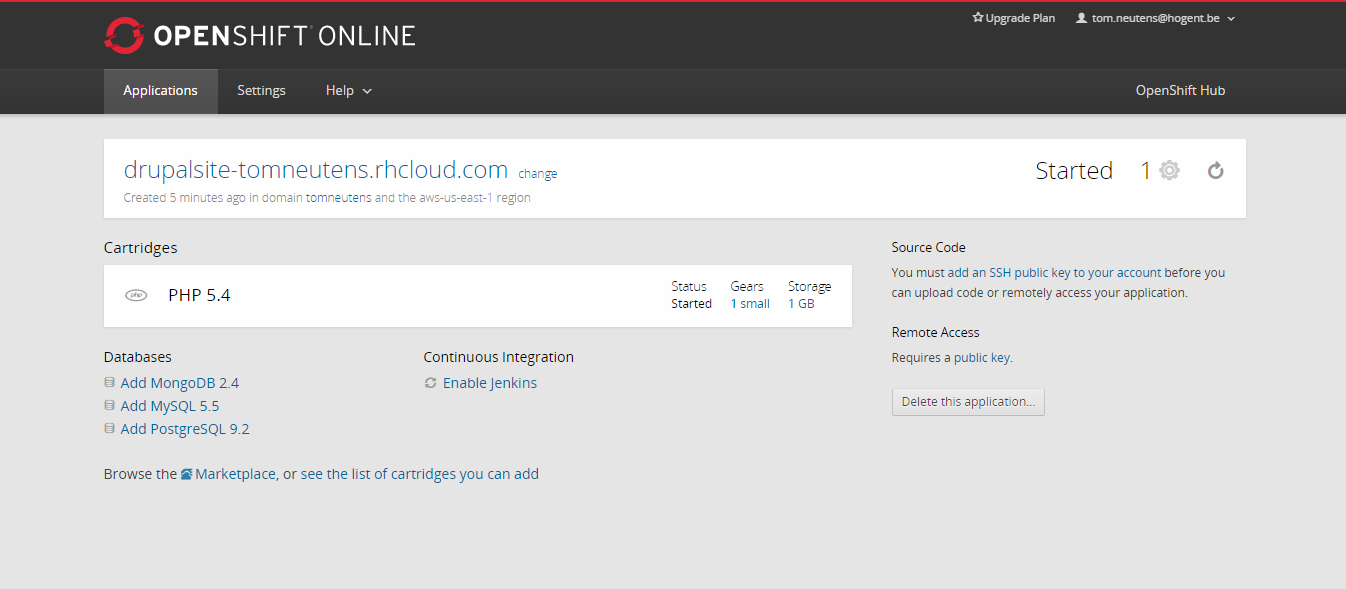
\includegraphics[width=\textwidth]{chapter7/openshift_applications_overview}
	\caption{OpenShift application overview page.}
	\label{fig:openshift_applications_overview}
\end{figure}

Since we are going to use a MySql database, click the \textbf{Add MySQL 5.5} link. On the next page click \textbf{Add Cartridge}. Make note of the database credentials, it's a good idea to take a screenshot! After adding the MySQL cartridge you should add the PHPMyAdmin cartridge to manage the database.

\section{Installing the OpenShift client tools}

To be able to manage your OpenShift site you have to install some tools. The following link (\url{https://developers.openshift.com/en/managing-client-tools.html}) gives step by step instructions on how to install them.

\section{Putting your site on openshift}

To start we will get a local copy of our application repository through git. Create the folder \url{C:/openshift_repos/bitingbugs_example} on your local machine. Navigate to the new folder through Windows explorer. Right click somewhere on the window and select \textbf{Git bash} (figure \ref{fig:git_contextual_menu}).  

\begin{figure}[H]
	\centering
	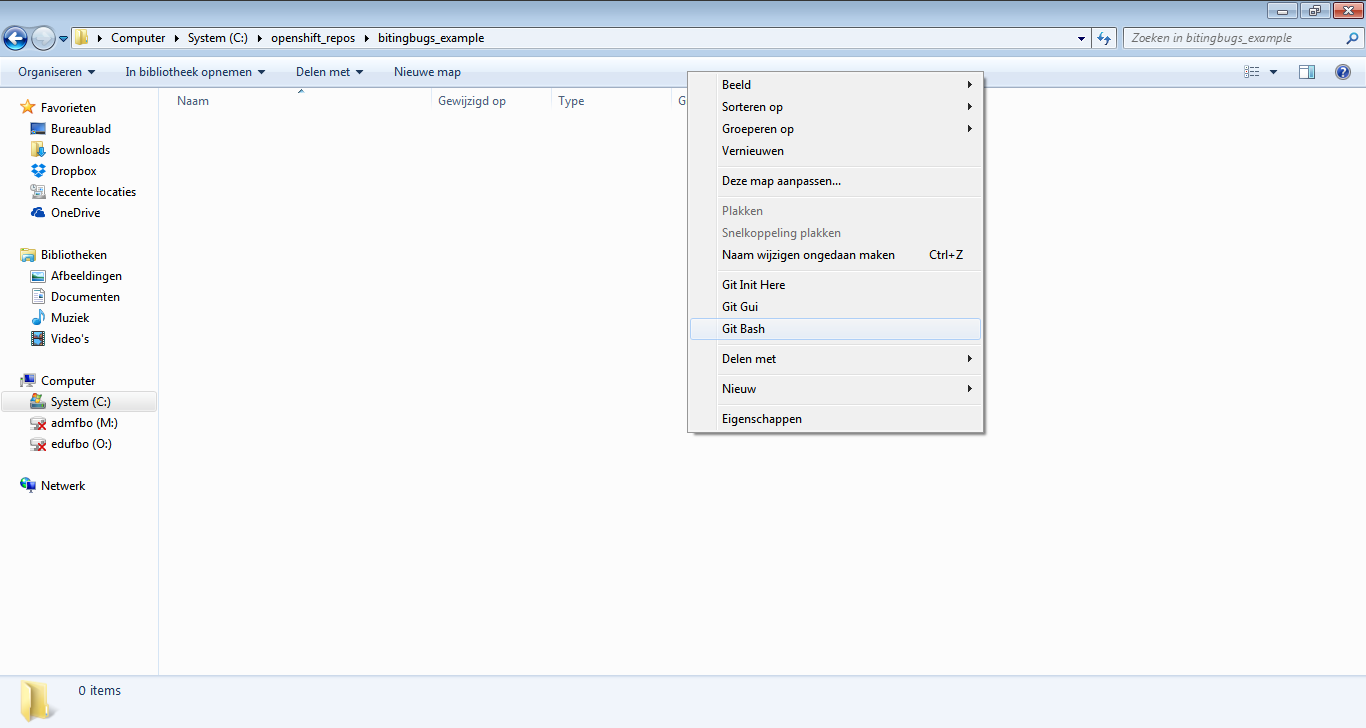
\includegraphics[width=\textwidth]{chapter7/git_contextual_menu}
	\caption{Open the Git bash shell.}
	\label{fig:git_contextual_menu}
\end{figure}

We are going to clone our OpenShift repository to our local machine. If u followed the steps in the previous section correctly, you should find the url to your repository on your OpenShift application page (Figure \ref{fig:openshift_applications_page}).

\begin{figure}[H]
	\centering
	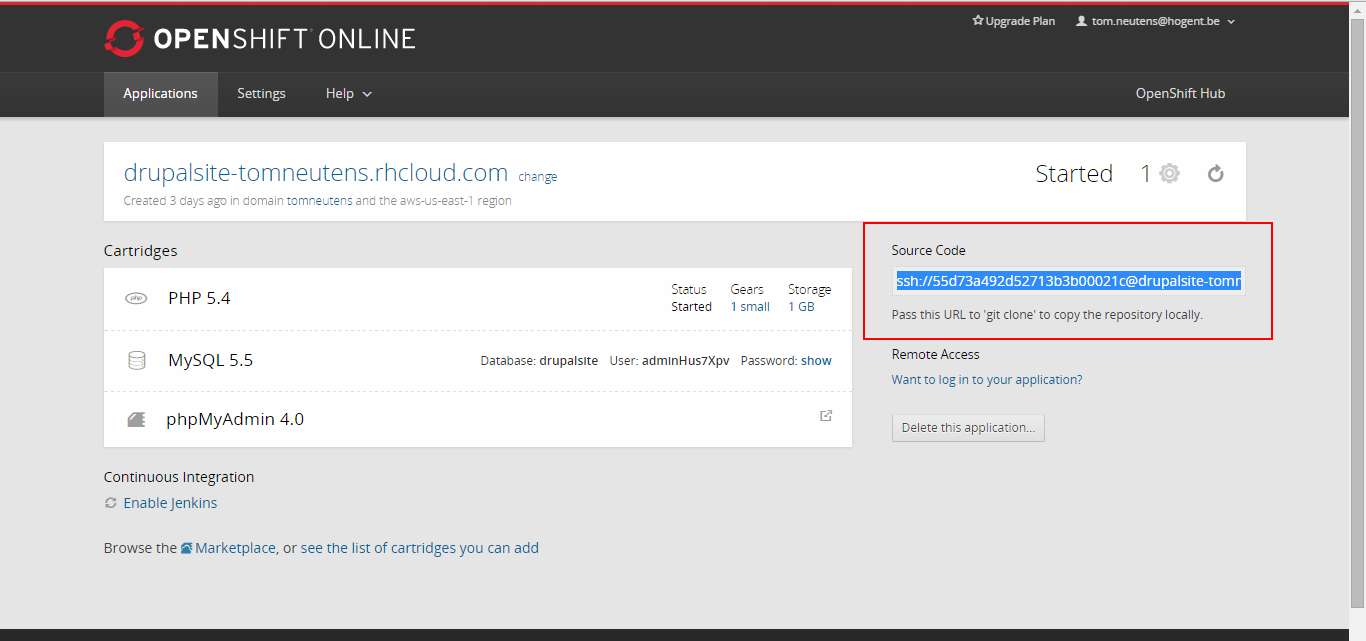
\includegraphics[width=\textwidth]{chapter7/openshift_applications_page}
	\caption{Open the Git bash shell.}
	\label{fig:openshift_applications_page}
\end{figure}

Go back to the Git bash shell and type the following command \textbf{git clone \textless git-url \textgreater}. This will create a local copy of your OpenShift code. For now this code is very limited. If you look in the \textbf{drupalsite} folder you will only see one file, the \url{index.php}. In the next step we are going to replace the \url{index.php} file by our Drupal site code. 
Go to the folder where you stored the code for the bitingbugs example (figure \ref{fig:local_codebase}) and copy it to your new repository (figure \ref{fig:local_openshift_repo}).

\begin{figure}[H]
	\centering
	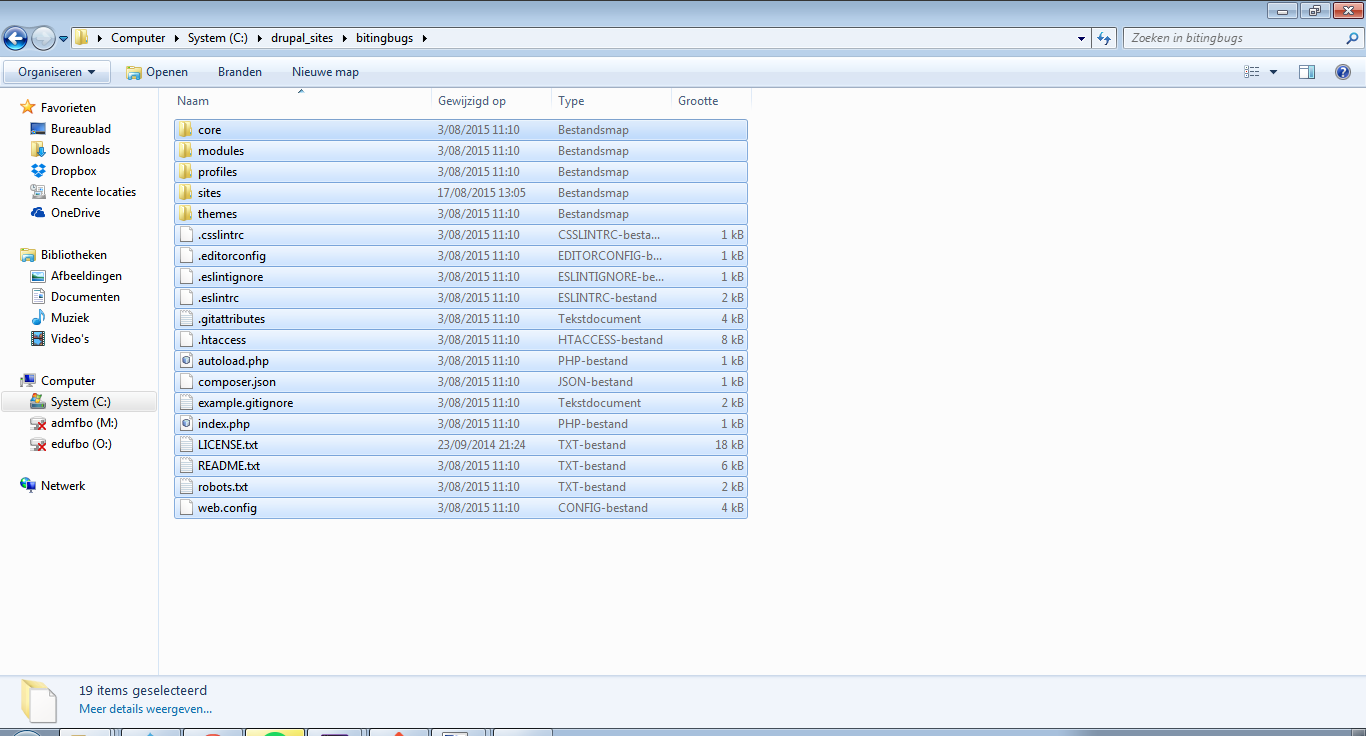
\includegraphics[width=\textwidth]{chapter7/local_codebase}
	\caption{The local codebase, this is the code managed by the Acquia Dev desktop.}
	\label{fig:local_codebase}
\end{figure}


 \begin{figure}[H]
 	\centering
 	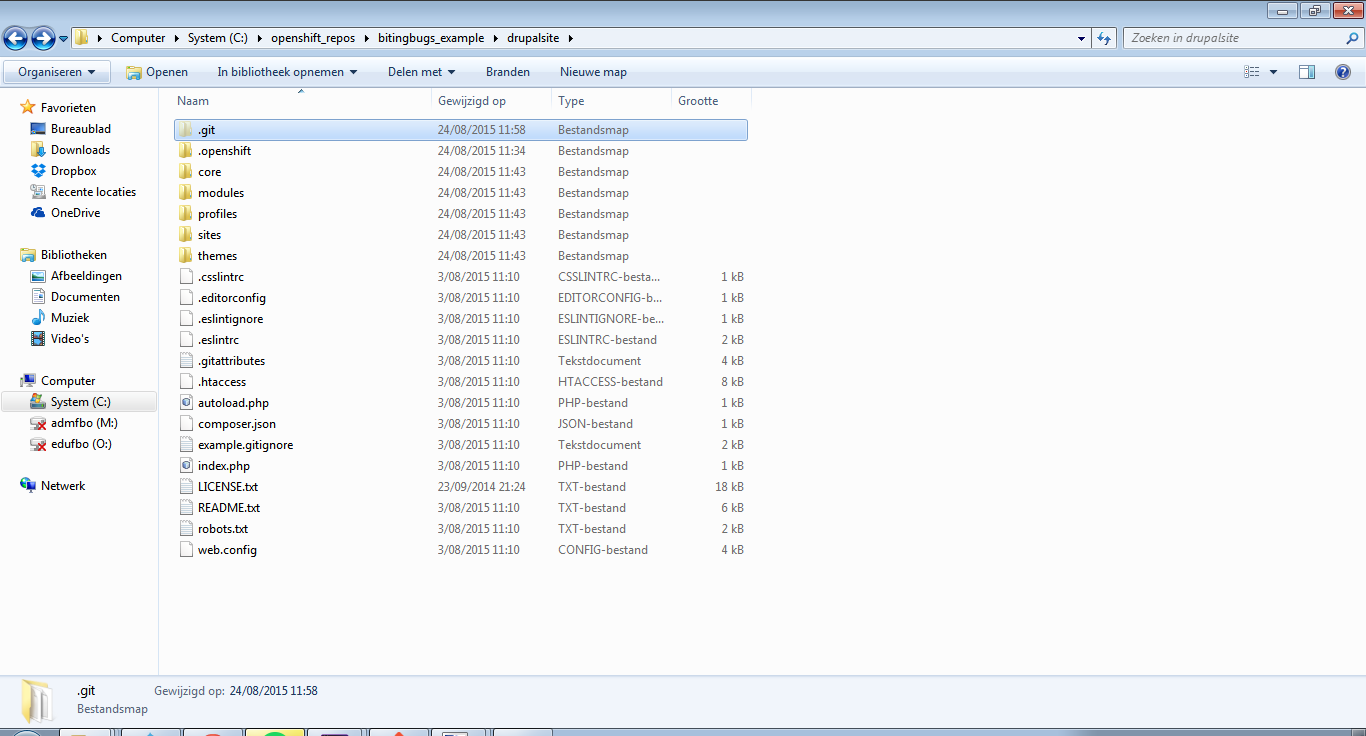
\includegraphics[width=\textwidth]{chapter7/local_openshift_repo}
 	\caption{The location of your OpenShift local git repository.}
 	\label{fig:local_openshift_repo}
 \end{figure}
 
 To add your Drupal site into the git versioning system go back to the \url{drupalsite} folder and execute the command \textbf{git add *}, this might take a while (figure \ref{fig:git_add_command}). You can use the \textbf{git status} command to see all the files that where added.
 
 \begin{figure}[H]
 	\centering
 	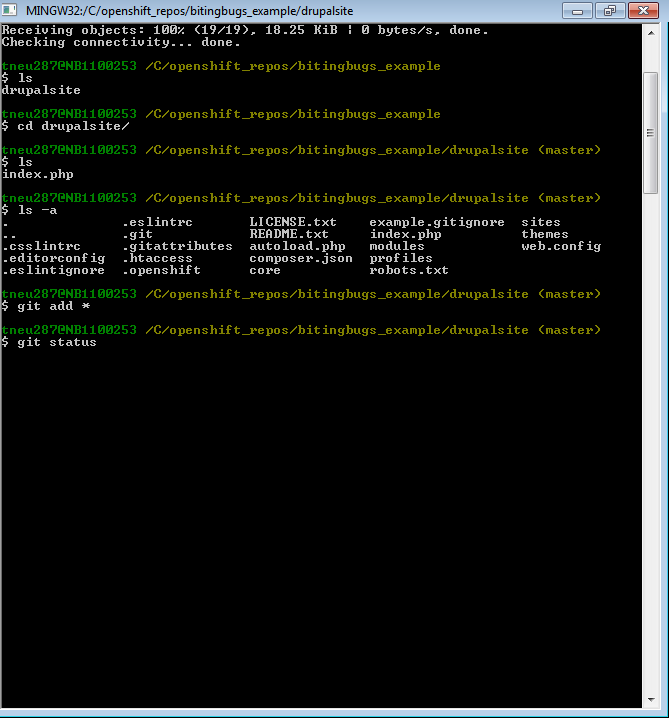
\includegraphics[width=\textwidth]{chapter7/git_add_command}
 	\caption{Git add command.}
 	\label{fig:git_add_command}
 \end{figure}
 
 After running the \textbf{git status} you should see the following result:
 
  \begin{figure}[H]
  	\centering
  	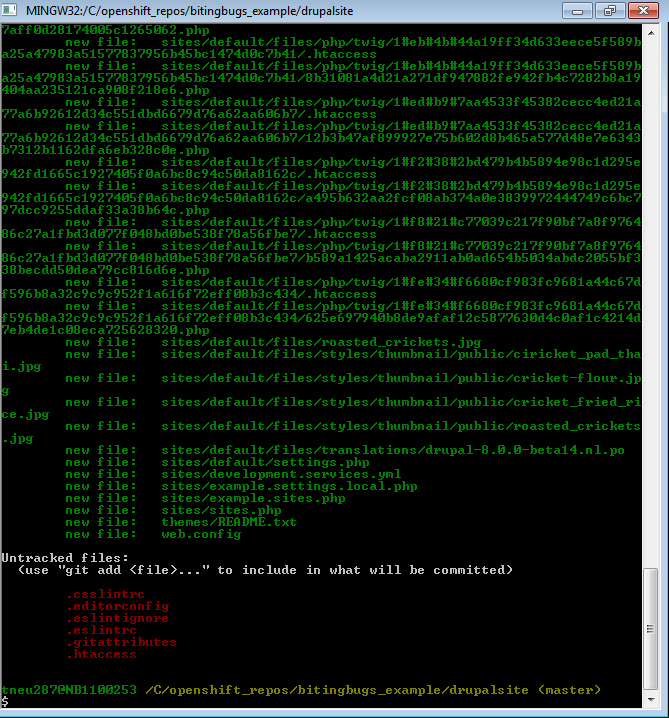
\includegraphics[width=\textwidth]{chapter7/git_status_command}
  	\caption{Git status command.}
  	\label{fig:git_status_command}
  \end{figure}
  
  As you can see some files are not added. To make sure routing works correctly you should add the \url{.htaccess} file. (\textbf{git add .htaccess}). Next we commit the new files to the local repository. Use \textbf{git commit -m "initial commit, adding all files"}. The \textbf{-m} parameter (commit message) is not mandatory but it is a good practice to always add it! 
  
  \section{Migrating your database to OpenShift}
  
  Our code has been uploaded to OpenShift but our OpenShift database is still empty. First we will make a dump of our local database, afterwards we will upload the data to our OpenShift database. To create the dump file go to the phpMyAdmin page of your local site. You can do this by clicking the link in the Acquia Dev desktop. Go to the \textbf{Export} tab and click the \textbf{Start} button. Next go to your OpenShift account and go to your application page. Click the link to the phpMyAdmin page (figure \ref{fig:openshift_phpmyadmin_link}). And enter your credentials (found on your application page).
  
    \begin{figure}[H]
    	\centering
    	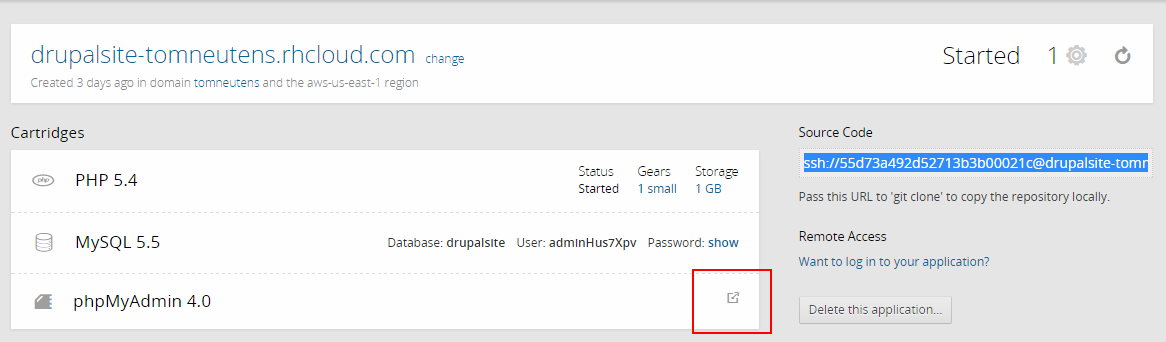
\includegraphics[width=\textwidth]{chapter7/openshift_phpmyadmin_link}
    	\caption{OpenShift phpMyAdmin link.}
    	\label{fig:openshift_phpmyadmin_link}
    \end{figure}
    
    When you are logged into your OpenShift phpMyAdmin page, first select the drupalsite database in the left menu. Next click the \textbf{import} tab. On the import page, select your local dump file and click the \textbf{Start} button.
    
    